%%%%%%%%%%%%%%%%%%%%%%%%%%%%%%%%%%%%%%%%%%%%%%%%%%%%%%%%%%%%%%%%%%%%%%%%%%%%%%%%
% Limit_Intepretation.tex: Select of showering and tracking events:
%%%%%%%%%%%%%%%%%%%%%%%%%%%%%%%%%%%%%%%%%%%%%%%%%%%%%%%%%%%%%%%%%%%%%%%%%%%%%%%%
\chapter{Limit Interpretation}
\label{Limit_Results_and_Intepretation_Chapter}
%%%%%%%%%%%%%%%%%%%%%%%%%%%%%%%%%%%%%%%%%%%%%%%%%%%%%%%%%%%%%%%%%%%%%%%%%%%%%%%%
The observed~($N^{Obs}$) confidence limit on the number of events is related to the expected~($N^{Expt}$) number of events from the SPS8 GSMB model through the relation
\begin{equation}{\label{eq:NUPA}}
 \mu^{UL} = \frac {N^{Obs}}{N_{Expt}}
\end{equation}
where, $\mu^{UL}$, is the upper limit on the signal strength obtained from running the HiggsCombine tool  with the $CL_{s}$ procedure.
Using the relationship between the cross section~($\sigma$) and the number of events~($N$): $\sigma = \frac{N}{\varepsilon\times A \cdot \mathscr{L}}$, and Equation \ref{eq:NUPA}, the observed upper limit on the cross section is evaluated in the following way
\begin{equation}{\label{eq:SIGMAUPA}}
\sigma^{Obs}_{UL} = \frac{\mu^{UL} \cdot N^{Expt}}{\varepsilon\times A\cdot \mathscr{L}}
\end{equation}
where, $\mathscr{L}$, is the integrated luminosity~(19\fbinv) and $\varepsilon$ and $A$ are the signal selection Efficiency and Acceptance, respectively.
\par 
In addition to the \textbf{observed} limit~(shown as a solid black line in Figure \ref{fig:SPS8_Ctau_Ulimit}), we also evaluate the uncertainties on the \textbf{expected} or median~(50\%) limit~(dashed red line) at 68\%~($+ 1\sigma$) or 16\%~($- 1\sigma$) and at 98\%~($+ 2\sigma$) or 2.5\%~($- 2\sigma$) shown with the \textcolor{green}{GREEN} and \textcolor{yellow}{YELLOW}  bands, respectively, in the same Figure \ref{fig:SPS8_Ctau_Ulimit}.
\newline
Using the cross section from theory~(shown as the blue line in Figure \ref{fig:SPS8_Ctau_Ulimit}, for example), the excluded region in the mean lifetime of the lightest neutralino according to the SPS8 benchmark GMSB model are the values of mean lifetime, $\tau$, for which the observed cross section is below the theory cross section, \ie a lower limit and an upper limit on $\tau$ is extracted which corresponds to the points where the observed cross section and the theory cross section intersect.
An exclusion  upper limit on the mass or effective SUSY breaking scale, $\mathbf{\Lambda}$, is obtained from Figure \ref{fig:limits} at the point where the observed cross section~(solid black line) intersects with the expected~(blue line) cross section. 
\newline
Using  the upper limits in $\tau$ and mass of neutralino or effective SUSY breaking scale, $\mathbf{\Lambda}$, we produce a two dimensional exclusion limit in $\tau$ and $\mathbf{\Lambda}$ and also a cross section limit according to the SPS8 benchmark GMSB model. 

%%%%%%%%%%%%%%%%%%%%%%%%%%%%%%%%%%%%%%%%%%%%%%%%%%%%%%%%%%%%%%%%%
\section{Signal Efficiency and Acceptance}
%%%%%%%%%%%%%%%%%%%%%%%%%%%%%%%%%%%%%%%%%%%%%%%%%%%%%%%%%%%%%%%%%
The plot in Figure \ref{fig:EffAcc} show our signal selection efficiency and acceptance for signal events of MC samples with different mean lifetime in \mm or \textit{proper decay length}, $c\tau$, ranging from 500\mm to 6000\mm with the same lightest neutralino mass of 255\GeVcc or effective SUSY breaking scale $\mathbf{\Lambda=180}$\TeV. 

\vspace{5mm}
\begin{minipage}{0.90\linewidth} 
\begin{center}
%\mbox{
%\includegraphics[width=0.49\textwidth,height=0.5\textwidth]
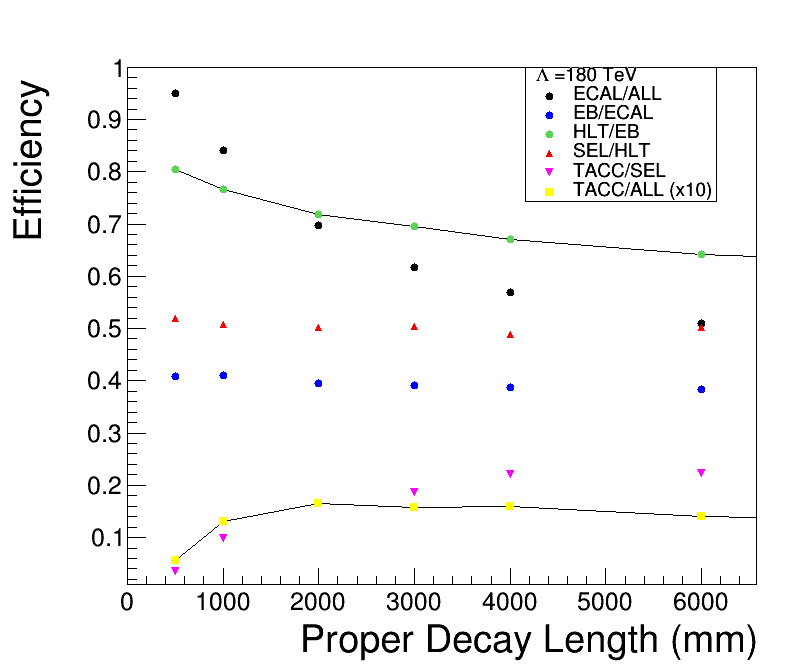
\includegraphics[height=0.65\textwidth, width=0.8\textwidth]{THESISPLOTS/Eff_180_ctau_2015.png}
%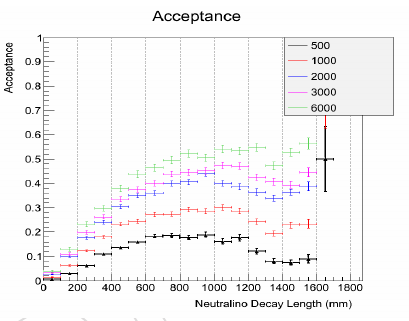
\includegraphics[height=0.5\textwidth, width=0.5\textwidth]{THESISPLOTS/SignalReconstructionAcceptance.png}}
\captionof{figure}{The efficiency against the mean decay length, $c\tau$ in \mm for $\mathbf{\Lambda=180}$\TeV. TACC/ALL~(yellow square markers) is the  Efficiency $\times$ Acceptance($t>3$~ns)~($\varepsilon \times A$) use in evaluating the exclusion limits. }
\label{fig:EffAcc}
\end{center}
\end{minipage}

\vspace{5mm}
The efficiency times acceptance~($\varepsilon \times A$) used in Equation \ref{eq:SIGMAUPA} to evaluate the exclusion limits is the TACC/ALL which is the ratio of the events passing our event selection with photon time, $t > 3$~ns in the barrel to all events with photons from the decay of the generated lightest neutralino. The $\times 10$  factor for TACC/ALL shown on the plot  is only for display purpose and was not used in evaluating the limits. 
\newline
The efficiency times acceptance, is small~(less than 10\%) for smaller values of $c\tau = 500\mm$~($\tau = 1.7$~ns) since very few of the events with photon from the lightest neutralino decay have time, $t > 3$~ns, despite many of photons reaching ECAL as is seen in the ECAL/ALL~(ratio of events with photons reaching ECAL to all events with photons from the decay of the generated lightest neutralino.) where the efficiency times acceptance is high for low $c\tau$ values. 
\newline
The efficiency times acceptance peaks at $c\tau = 2000\mm$~($\tau = 6.7$~ns) and then begins to slightly fall for larger $c\tau$ values. For very large $c\tau > 6000\mm$ values not shown on the plots, the efficiency times acceptance is again less than 10\% since most of the lightest neutralinos decay outside of the ECAL and are undetected, as seen in the ECAL/ALL where the efficiency keeps dropping with increased $c\tau$ values.

\section{Limits on SPS8 GMSB Model}
With the one event observed in our signal region passing our final event selection and acceptance, obviously not a significant excess over our estimated $0.37$ background events, we obtain an upper limit on the event photon count of $4.07$ at 95\% CL using the $CL_{s}$ procedure. This upper limit in the event count is obtained using maximum number of signal events expected of $2.95$ in a negligible background events with a theoretical cross section of 1.0~fb for total integrated luminosity of 19.1\fbinv. 
If  the effective SUSY breaking scale according to the SPS8 benchmark GMSB model is $\mathbf{\Lambda} = 180\TeV$, corresponding to a lightest neutralino production cross section and decay to photon and gravitino, $\PSneutralinoOne \rightarrow \gamma + \tilde{G}$, channel of 12.05~fb \ie $\sigma\times BR = 12.05$~fb, the mean lifetime of the lightest neutralino, $\tau_{\PSneutralinoOne}$, is either  less than $3.2$~ns or larger than 19.87~ns as shown in right plot of Figure \ref{fig:SPS8_Ctau_Ulimit}.

\vspace{5mm}
\begin{minipage}{0.90\linewidth}
\begin{center}
%\mbox{
%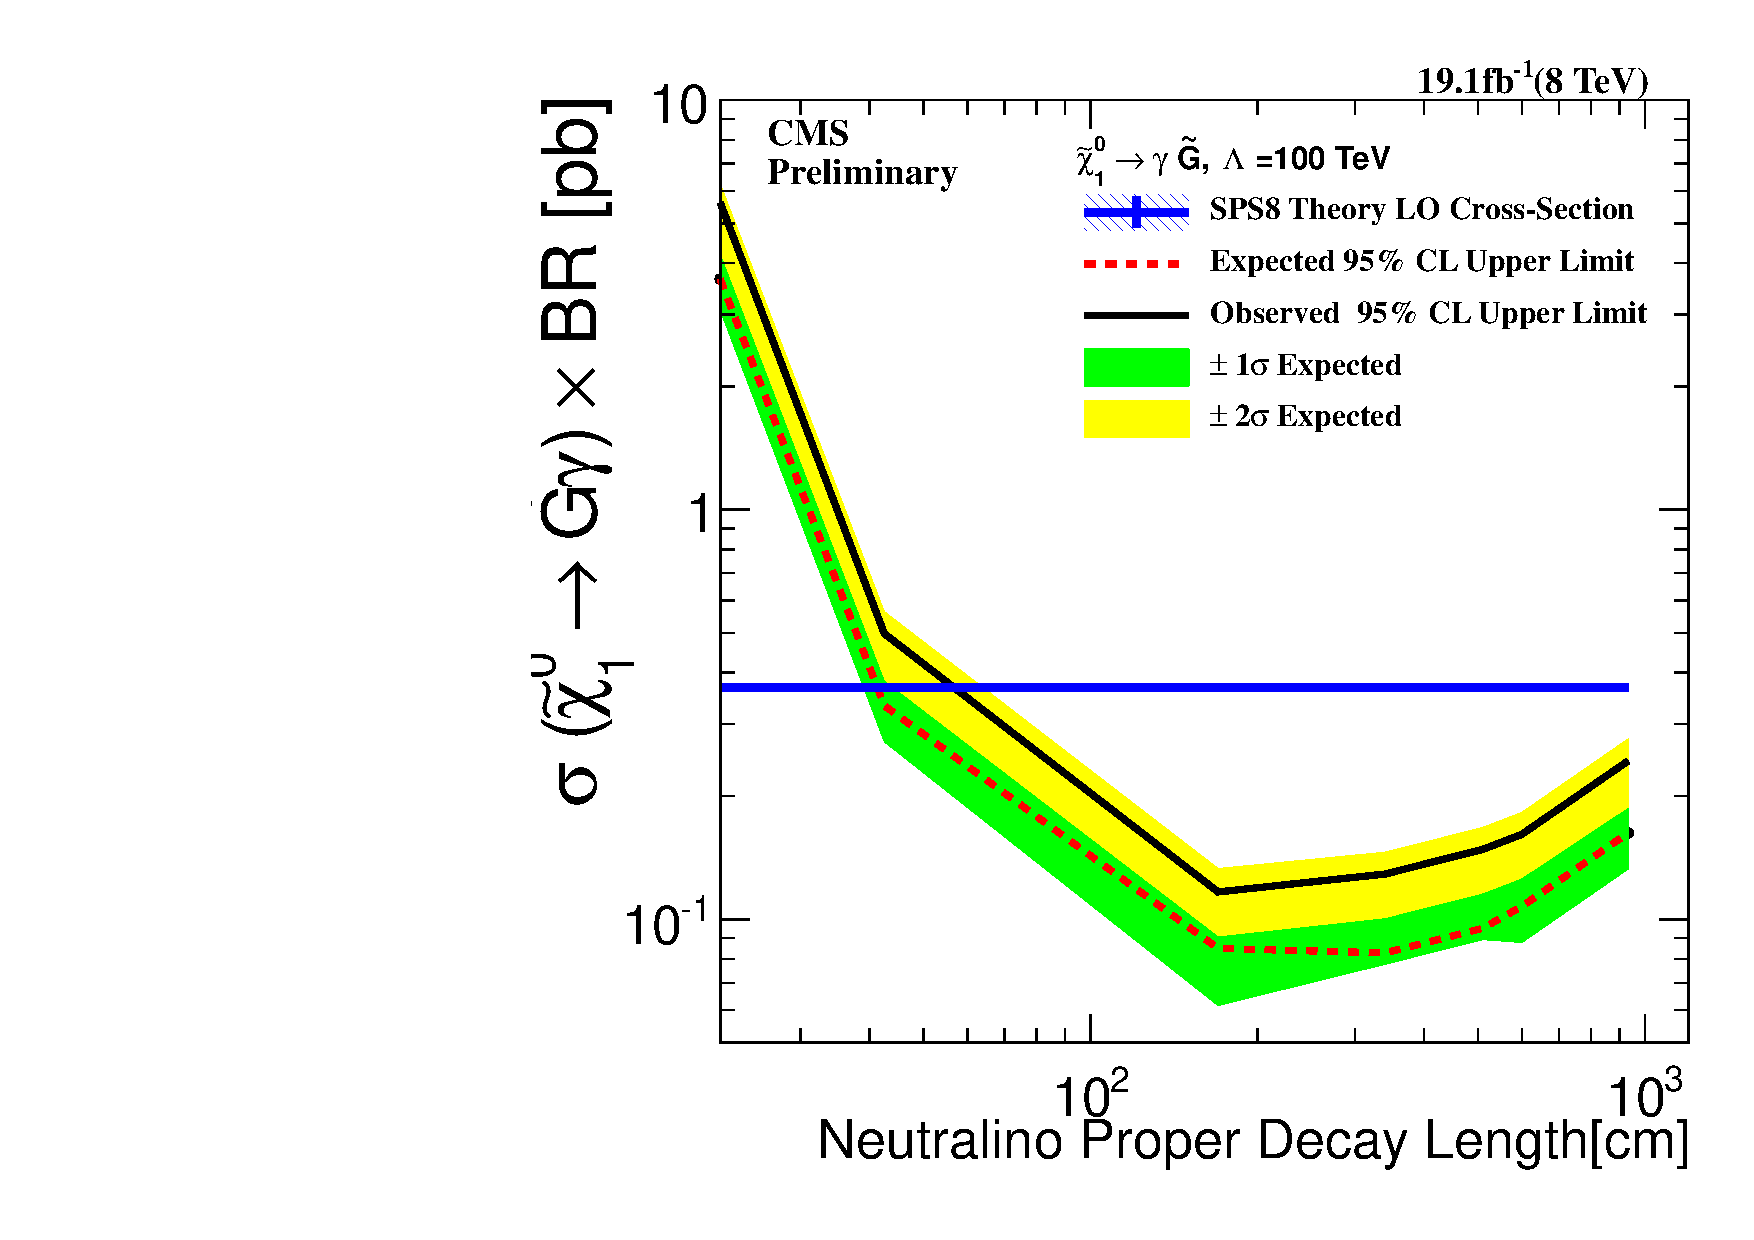
\includegraphics[height=0.65\textwidth, width=0.53\textwidth]{THESISPLOTS/100TeV_Neutralino_CrossSecTimesBR_Uplimit.pdf}
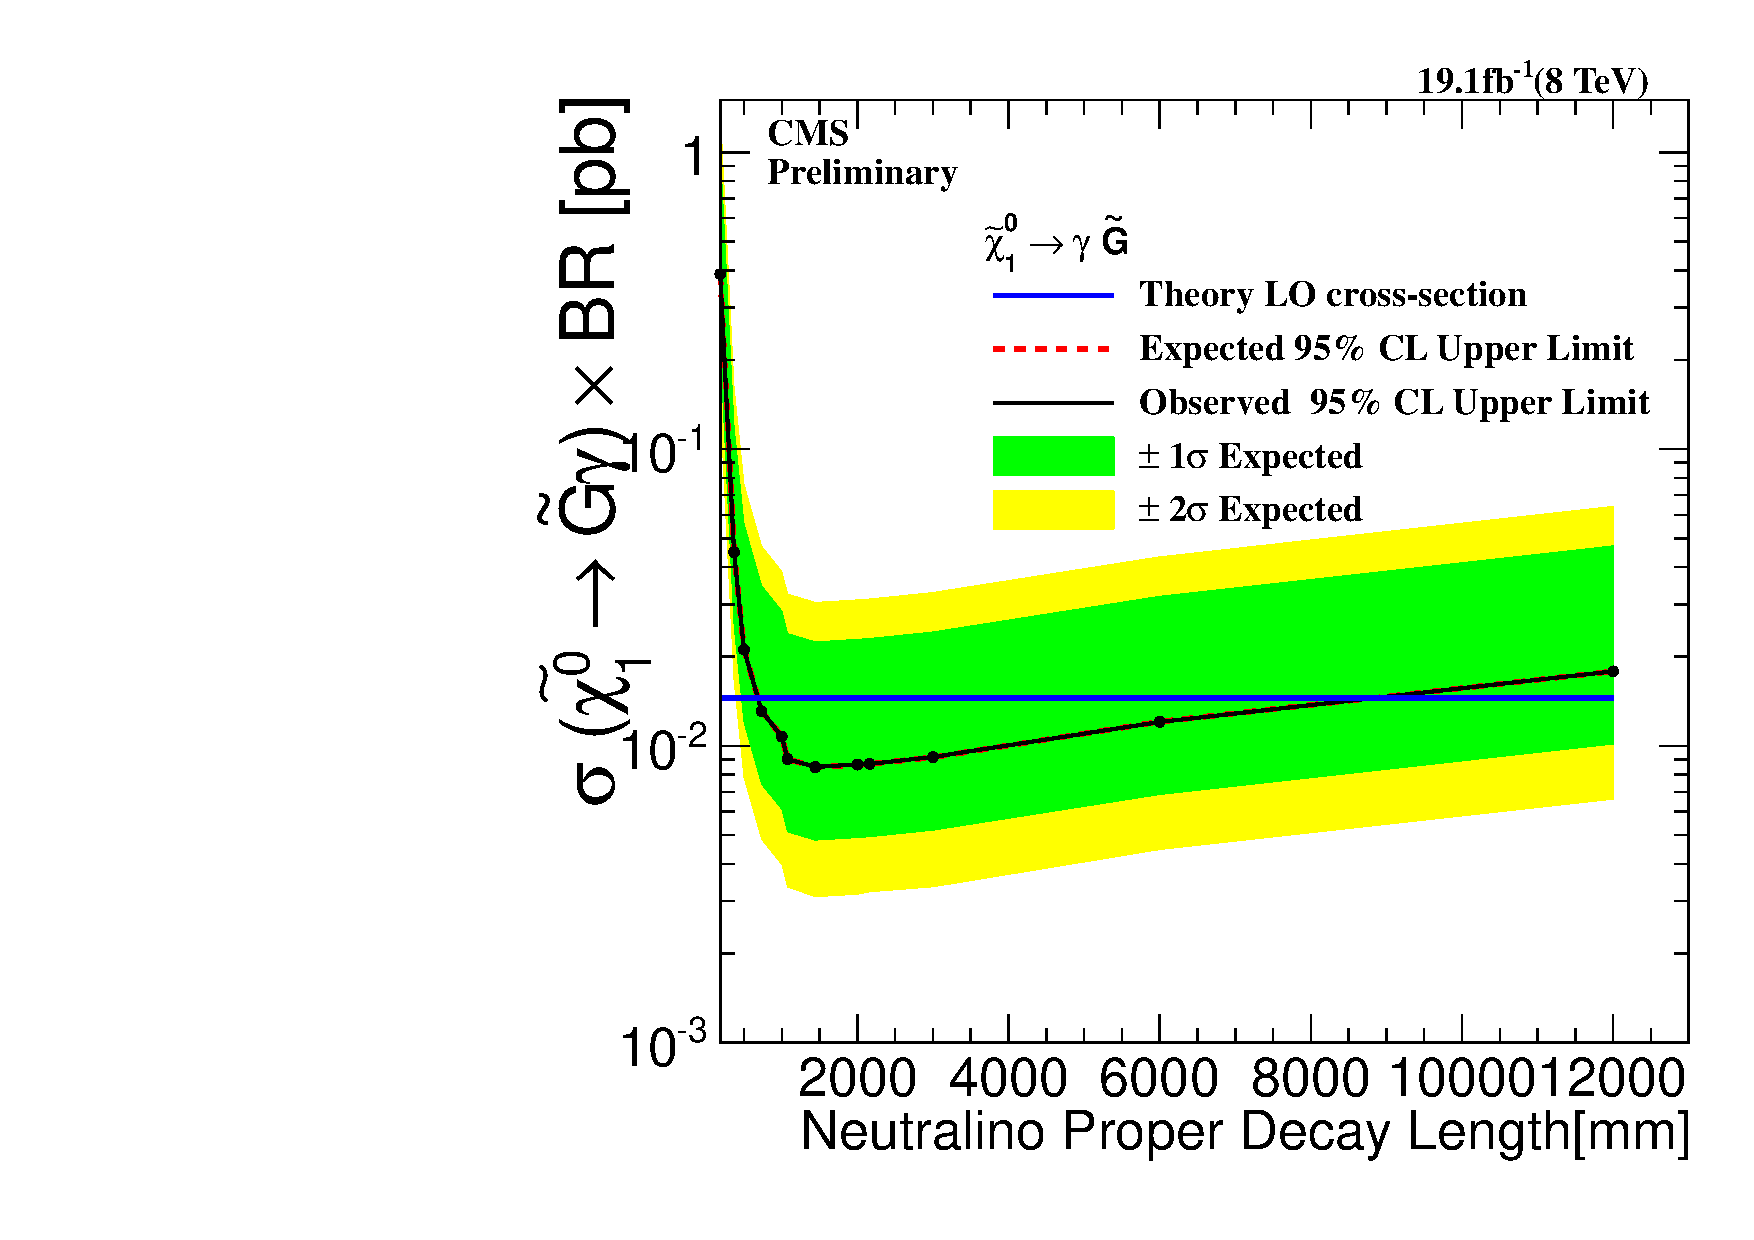
\includegraphics[height=0.8\textwidth, width=0.85\textwidth]{THESISPLOTS/Neutralino_CrossSecTimesBR_Uplimit.pdf} 
%}
\captionof{figure}{ 95\% CL evaluated using the $CL_{s}$ procedure on the lightest neutralino production cross section times branching ratio~($\sigma\times BR$) against mean lifetime~(ns) for $\mathbf{\Lambda = 180}$\TeV in the SPS8 benchmark GMSB model.}
\label{fig:SPS8_Ctau_Ulimit}
\end{center}
\end{minipage}
\vspace{5mm}

The excluded lightest neutralino mass, $m_{\PSneutralinoOne}$, or effective SUSY breaking scale, $\mathbf{\Lambda}$, observed from the cross section against lightest neutralino mass plot of Figure \ref{fig:MASS-limits} for $\tau = 6.7$~ns is up to  $m_{\PSneutralinoOne} = 300\GeVcc$ or  $\mathbf{\Lambda} = 220\TeV$, still in the context of the SPS8 benchmark GMSB model.
\newline
From the 2 dimensional plane define by $(\mathbf{\Lambda},\tau_{\PSneutralinoOne})$ of the exclusion limit, shown in  Figure \ref{fig:SPS8_2D-Ulimit}, the excluded lightest neutralino mean lifetime, $\tau_{\PSneutralinoOne}$, is from $2.0$~ns to $45.0$~ns for low mass~($m_{\PSneutralinoOne} < 150\GeVcc$) lightest neutralino. This exclusion in mean lifetime shrinks as the mass of the lightest neutralino increases or effective SUSY breaking scale increases. This is because the production cross section for the lightest neutralino decreases with increase in its mass or $\mathbf{\Lambda}$. 
\newline
For a given lightest neutralino mass and mean lifetime, we can also find its corresponding excluded cross section using Figure \ref{fig:SPS8_SIGMA-Ulimit}. For example, lightest neutralinos with mass,  $m_{\PSneutralinoOne} = 255\GeVcc$, or effective SUSY breaking scale,  $\mathbf{\Lambda} = 180\TeV$, and mean lifetime, $\tau_{\PSneutralinoOne} = 10.0$~ns, have an observed upper limit on their production cross section times branching ratio in the decay to photon and gravitino channel of $\sigma^{UP}_{\PSneutralinoOne} \geq 0.01$~pb at 95\% CL.

\vspace{5mm}
%\begin{figure}[!htb]
\begin{minipage}{0.90\linewidth}
%%\afterpage{ %
 %% \clearpage% Flush earlier floats (otherwise order might not be correct)
   %% \thispagestyle{empty}% empty page style (?)
%%\begin{landscape}% Landscape page
\begin{center}
%\mbox{
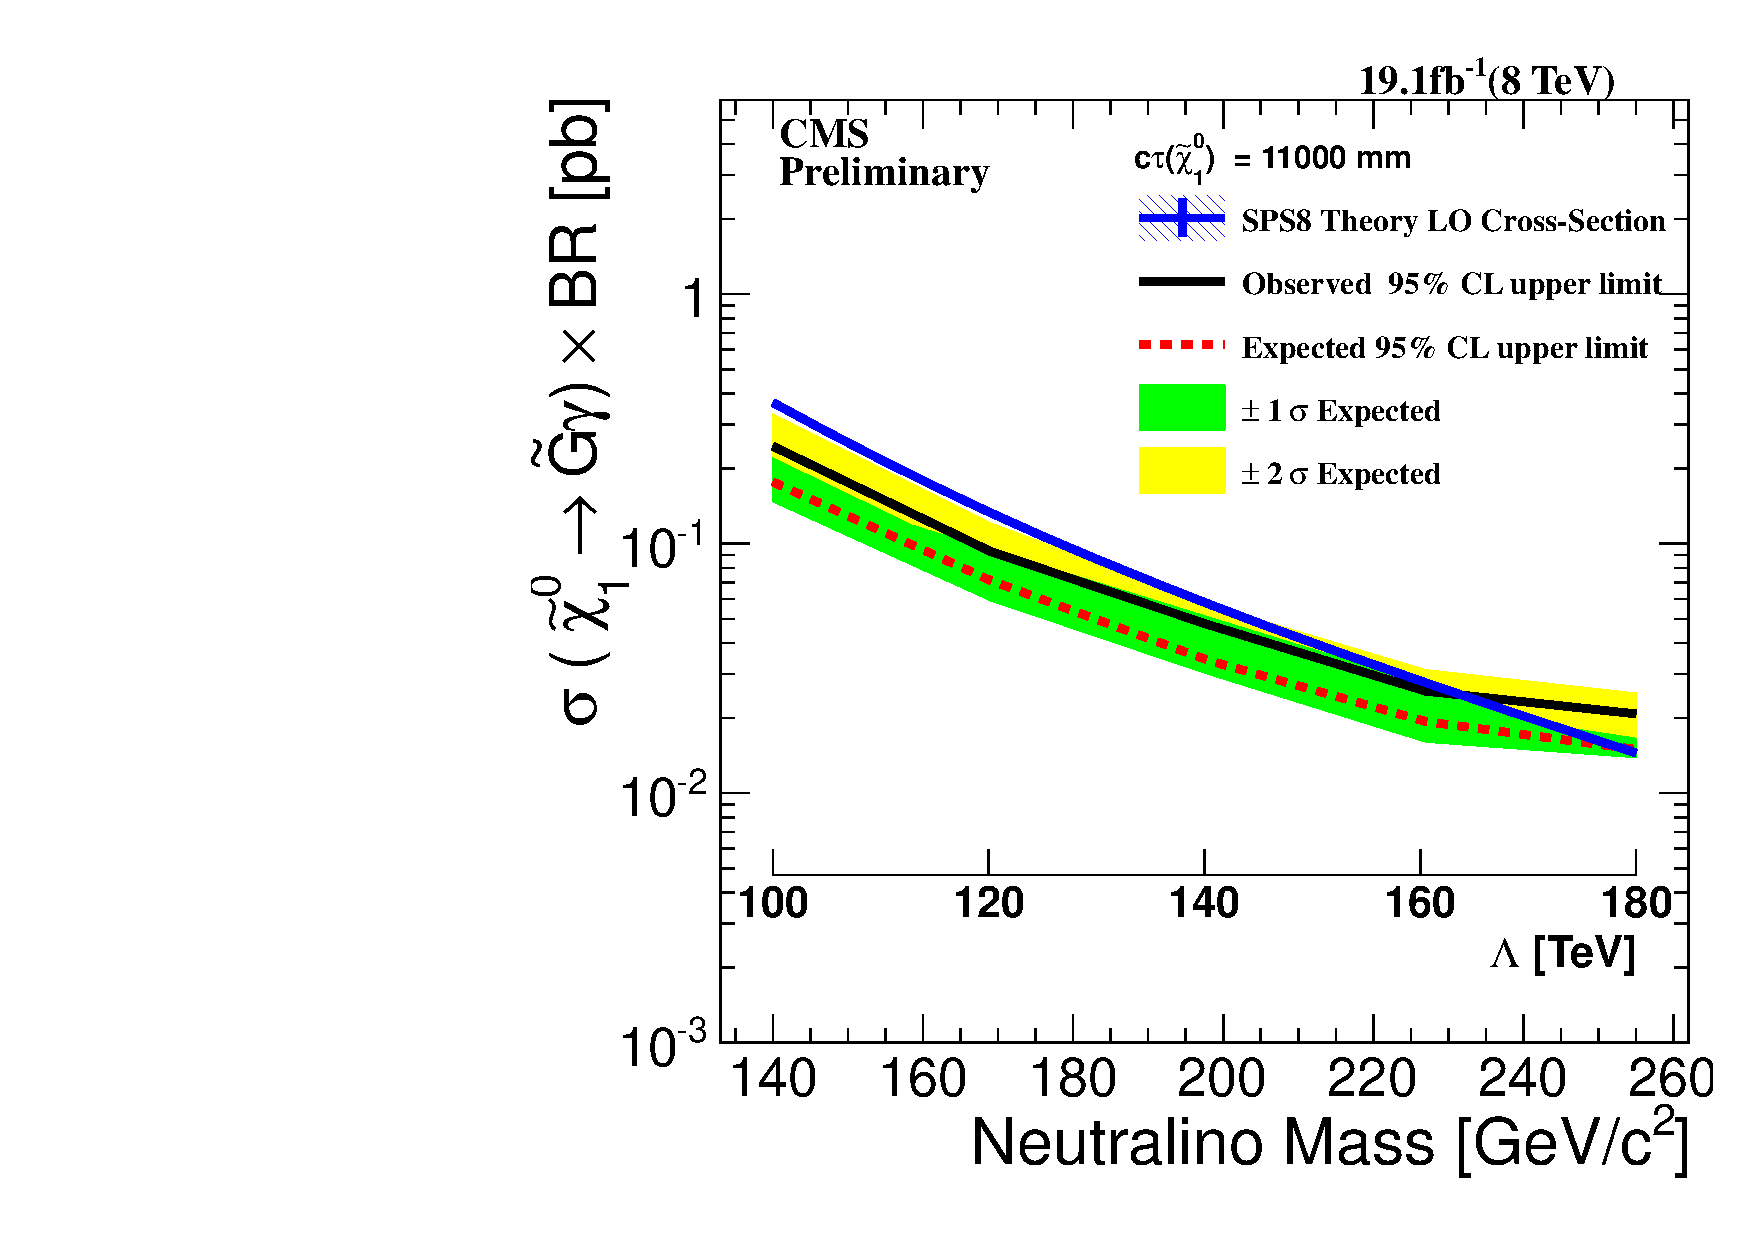
\includegraphics[height=0.8\textwidth, width=0.85\textwidth]{THESISPLOTS/Neutralino_CrosSecVsMass_Exclusion_limit_11000.pdf}
%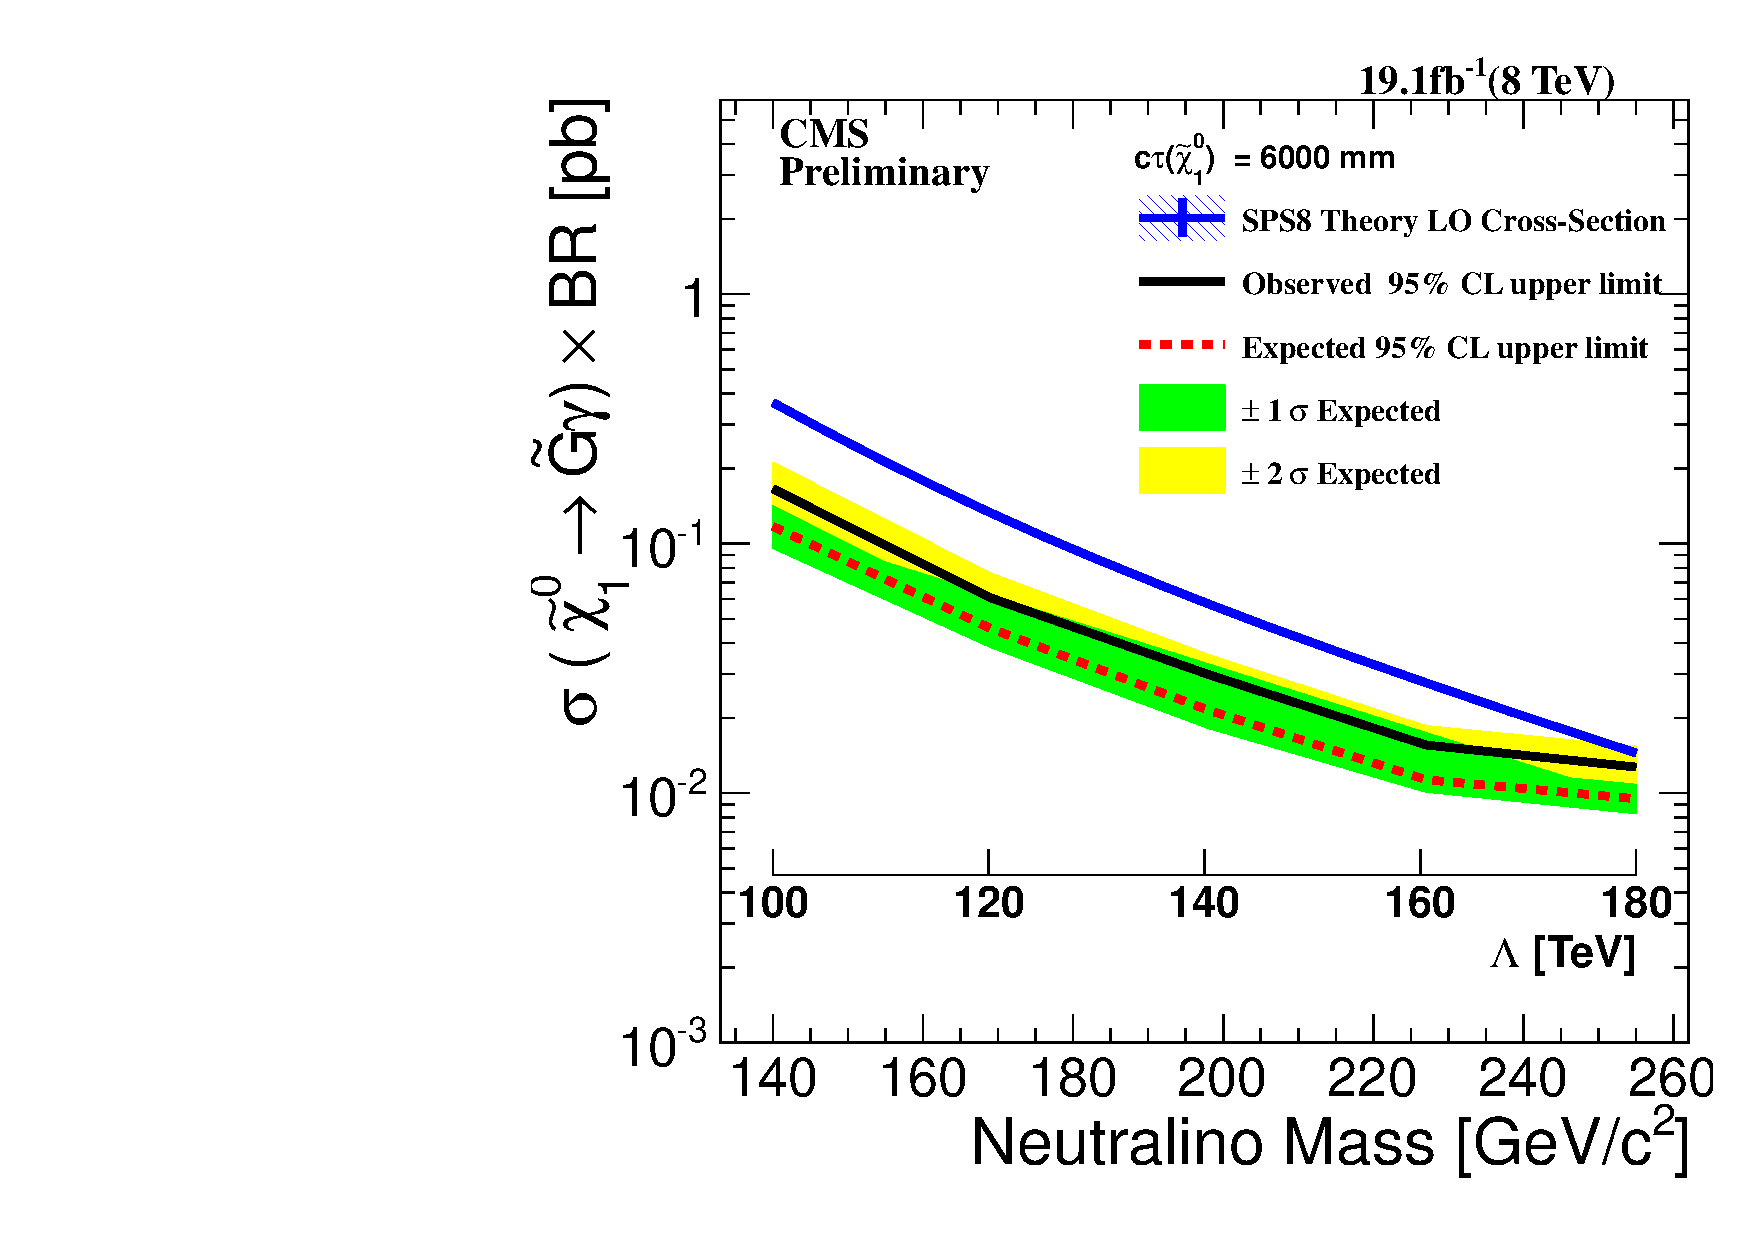
\includegraphics[height=0.65\textwidth, width=0.53\textwidth]{THESISPLOTS/Neutralino_CrosSecVsMass_Exclusion_limit_6000.pdf} }
\captionof{figure}{95\% CL evaluated using the $CL_{s}$ procedure on the lightest neutralino production cross section times branching ratio~($\sigma\times BR$) for different $\mathbf{\Lambda}$~(or mass of lightest neutralino) for $c\tau = 11000\mm$ or $\tau = 36.7$~ns in the SPS8 benchmark GMSB model.}
\label{fig:MASS-limits}
\end{center}
%\end{figure}
\end{minipage}
\vspace{5mm}

\begin{minipage}{0.95\linewidth}
\begin{center}
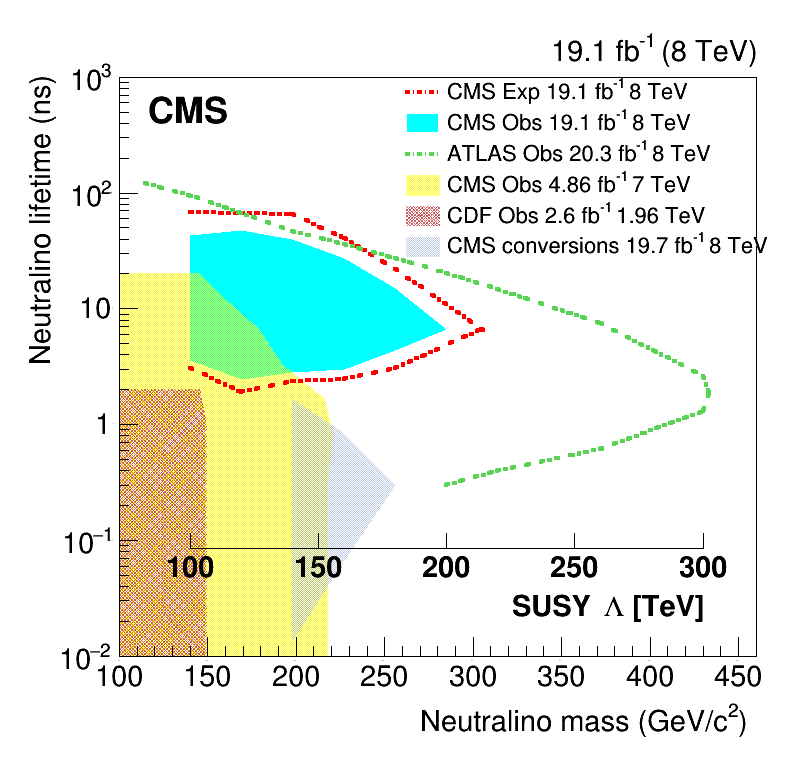
\includegraphics[height=0.85\textwidth, width=0.9\textwidth]{THESISPLOTS/Exclude2D_withAtlas_2015.png}
\captionof{figure}{95\% CL exclusion limit in lightest neutralino mass~(or $\mathbf{\Lambda}$) against mean lifetime in SPS8 benchmark GMSB model. Limits from previous experiments also shown.}
\label{fig:SPS8_2D-Ulimit}
\end{center}
\end{minipage}
\vspace{5mm}

\begin{minipage}{0.95\linewidth}
\begin{center}
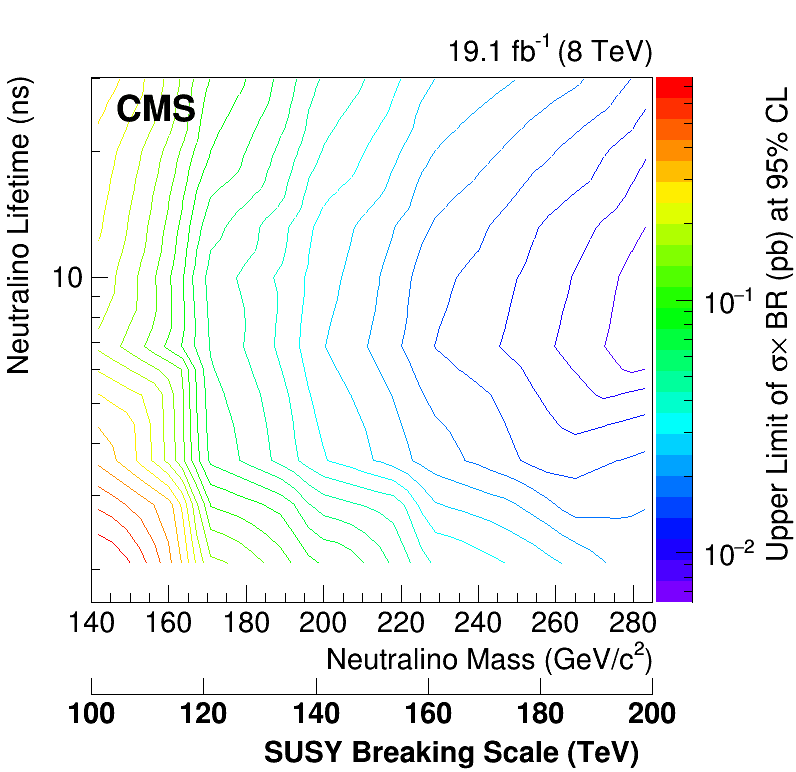
\includegraphics[height=0.85\textwidth, width=0.9\textwidth]{THESISPLOTS/limit2D_Cross-Section-Observed.png}
\captionof{figure}{95\% CL in cross section for different mass and lifetime of the lightest neutralino using the 8\TeV data corresponding to an integrated luminosity of 19.1\fbinv of the CMS experiment.}
\label{fig:SPS8_SIGMA-Ulimit}
\end{center}
\end{minipage}
%%\end{landscape}
%% \clearpage% Flush page
%%}

%%%%%%%%%%%%%%%%%%%%%%%%%%%%%%%%%%%%%%%%%%%%%%%%%%%%%%%%%%%%%%%%%%%%%%%%%%%%%%%%%%%%%%%%%%%%%%%%%%%%%%%
%%%%%%%%%%%%%%%%%%%%%%%%%%%%%%%%%%%%%%%%%%%%%%%%%%%%%%%%%%%%%%%%%%%%%%%%%%%%%%%%%%%%%%%%%%%%%%%%%%%%%%%

\begin{comment}
%%is given in table \ref{tab:SIGNALRES}
%%\vspace{5mm}
%%\begin{minipage}{\linewidth} 
%%\begin{center}
%\begin{table}[ht]
%\renewcommand\arraystretch{1.2}
%%\begin{tabular}{c c}
%%\toprule
%%\hline
%%\bfseries{SPS8 GMSB Signal} & \bfseries {Number of Events}\\
%%\hline
%%\toprule
%%\texttt{GMSB(SPS8)}~($\Lambda=180$~TeV,$c\tau=250$~mm) & $0.2096$ \\
%%\texttt{GMSB(SPS8)}~($\Lambda=180$~TeV,$c\tau=500$~mm) & $4.5423$  \\
%%\texttt{GMSB(SPS8)}~($\Lambda=180$~TeV,$c\tau=1000$~mm) & $6.3646$ \\
%%\texttt{GMSB(SPS8)}~($\Lambda=180$~TeV,$c\tau=2000$~mm) & $6.3968$ \\ 
%%\texttt{GMSB(SPS8)}~($\Lambda=180$~TeV,$c\tau=4000$~mm) & $6.1442$ \\
%%\texttt{GMSB(SPS8)}~($\Lambda=180$~TeV,$c\tau=6000$~mm) & $4.6498$ \\
%%\texttt{GMSB(SPS8)}~($\Lambda=180$~TeV,$c\tau=12000$~mm) & $2.918$ \\
%%\hline 
%%\bottomrule
%%\end{tabular}
%%\captionof{table}{Final number for $\Lambda = 180$\TeV GMSB SPS8 MC signal events  events passing our selection cuts.}
%%\label{tab:SIGNALRES}
%\end{table}
%%\end{center}
%%\end{minipage}
\end{comment}

%%%%%%%%%%%%%%%%%%%%%%%%%%%%%%%%%%%%%%%%%%%%%%%%%%%%%%%
%%%%%%%%%%%%%%%%%%%%%%%%%%%%%%%%%%%%%%%%%%%%%%%%%%%%%%%%%%%%%%%%%%%%%%%%%%%%%%%%
% Possible Future Analysis work!
%%%%%%%%%%%%%%%%%%%%%%%%%%%%%%%%%%%%%%%%%%%%%%%%%%%%%%%%%%%%%%%%%%%%%%%%%%%%%%%%
%\section{Future Improvements}
%%%%%%%%%%%%%%%%%%%%%%%%%%%%%%%%%%%%%%%%%%%%%%%%%%%%%%%%%%%%%%%%%%%%

%%%%%%%%%%%%%%%%%%%%%%%%

%\subsection{Beam Halo Monitoring Detector}
%\label{Beam Halo Procedure}
%%%%%%%%%%%%%%%%%%%%%%%%%%%%%%%%%%%%%%%%%%%%%%%%%%%%%%%%%%%%%%%%%%%%%%%%%%%%%%%%


%%%%%%%%%%%%%%%%%%%%%%%%%%%%%%%%%%%%%%%%%%%%%%%%%%%%%%%%%%%%%%%%%%%%%%%%%%%%%%%%
%\subsection{Back-end Electronics upgrade HCAL}
%\label{hcal)back_end_Electronics}

%%%%%%%%%%%%%%%%%%%%%%%%%%%%%%%%%%%%%%%%%%%%%%%%%%%%%%%%%%%%%%%%%%%%%%%%%%%%%}}}
